\documentclass[journal]{IEEEtran}

% *** CITATION PACKAGES ***
\usepackage[style=ieee]{biblatex} 
\bibliography{random_walk.bib}

% *** MATH PACKAGES ***
\usepackage{amsmath}

% *** PDF, URL AND HYPERLINK PACKAGES ***
\usepackage{url}
\hyphenation{op-tical net-works semi-conduc-tor}
\usepackage{graphicx}  % needed to include png, eps figures
\usepackage{float}  % used to fix location of images i.e.\begin{figure}[H]

% *** MY PACKAGES ***
\usepackage{todonotes}
\usepackage[caption=false]{subfig}

\begin{document}

% paper title
\title{Using Random Walk Simulations to Calculate Ground State Energies in
  Quantum Physics}

% author names 
\author{Sai Pandian, ID: 29899923}%
        
% The report headers
\markboth{PHYS6017 Computer Techniques in Physics Report 1, April 2020}
{Shell \MakeLowercase{\textit{et al.}}: Bare Demo of IEEEtran.cls for IEEE Journals}

% make the title area
\maketitle

% As a general rule, do not put math, special symbols or citations
% in the abstract or keywords.
\begin{abstract}
% Provide a summary of the session. What was done, what measurements were taken,
% brief methods, what calculations, brief conclusion.  The Abstract should be
% approximately 250 words or fewer, italicized, in 10-point Times (or Times
% Roman.) Please leave two spaces between the Abstract and the heading of your
% first section.  It should briefly summarize the essence of the paper and address
% the following areas without using specific subsection titles. Objective: Briefly
% state the problem or issue addressed, in language accessible to a general
% scientific audience. Technology or Method: Briefly summarize the technological
% innovation or method used to address the problem. Results: Provide a brief
% summary of the results and findings. Conclusions: Give brief concluding remarks
% on your outcomes. Detailed discussion of these aspects should be provided in the
% main body of the paper.
\end{abstract}


\section{Introduction}
\IEEEPARstart{T}{he} developments in computer power in recent years has opened
up the possibility for novel computational solutions to many problems that were
otherwise limited. We now have access to computers that can numerically solve
problems and run simulations that were previously too computationally intensive
to do.

One such problem is the calculation of the ground state energies of different
quantum systems. Many methods exist for solving these problems, using both
classical and quantum computational approaches. Whilst generally it may be true
that Quantum computating approahes are more suited to solving such problems
\cite{Mazzola}, these approaches are still in infancy and are not readily
accessible. Thus, there exist an abundance of classical computing approaches,
such as the Variational-Relaxiation algorithm \cite{Schroeder2017}. This is a
particularly useful algorithm for two-dimensional systems with non-separable
potentials but quickly becomes difficult to implement for more complex systems.

In this investigation, I explore an alternative Monte Carlo method using Random
Walk simulations, and demonstrate its efficacy with simple systems.


\section{Theoretical Background}
\label{sec:TheoreticalBackground}

\subsection{Random Walk Simulations}

Random walks descibe motion as a series of steps in some vector space, with the
direction of each step being random, i.e. with there being an equal likelihood
of a step in each possible direction. Consider a simple 1-dimensional line and a
walker standing at a point labelled the origin. The walker takes 20 steps, the
direction of each step (forwards or backwards on the line) is random. The
position of the walker at each step is shown in Figure \ref{fig:cartoon}.

\begin{figure}%[H]%%[!ht]
  \begin{center}
    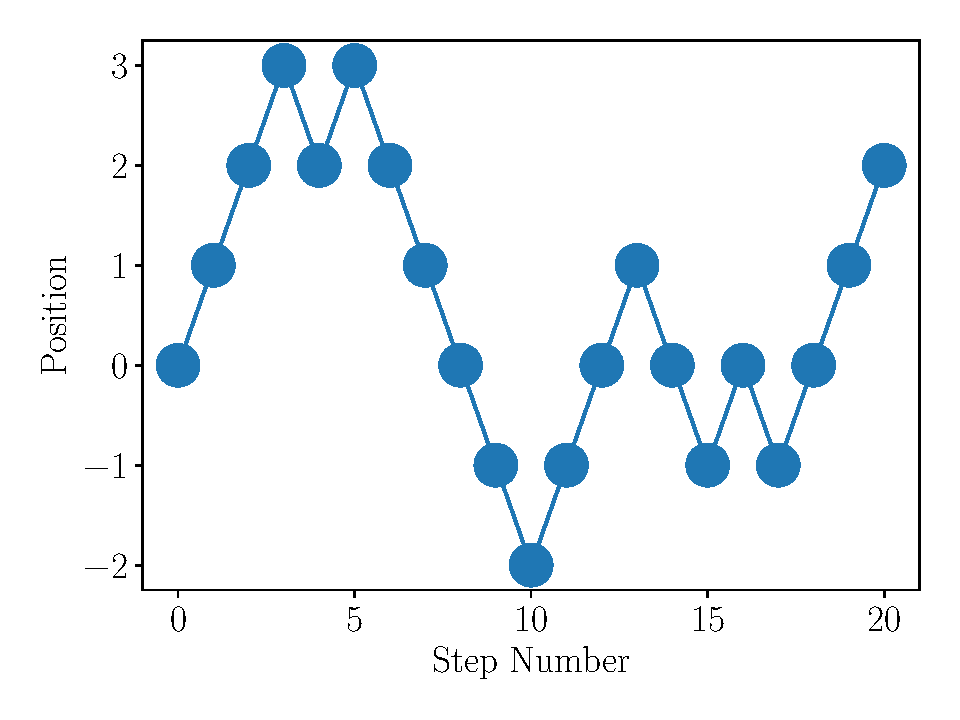
\includegraphics[width=0.45\textwidth]{images/cartoon.pdf}
    \caption{The position of a walker at each step in a 20-step random walk
      simulation. The average position of the walker does not necessarily remain
      at the origin as one might naively expect. Instead it is normal for the
      walker to finish the walk at some distance from the origin, as shown here.}
    \label{fig:cartoon}
  \end{center}
\end{figure}

As we can see from the figure, it is not uncommon for the average position of
the walker to be away from the origin once the walk has concluded. This is
because the position of the walker at any step is dependent only on the position
at the previous step. If the walker happens to take a number of steps in the
same direction, it is highly unlikely for the walker to take an equal number of
steps in the opposite direction, in order to return to the origin. Thus, in such
a case, it is likely that the walker will conclude the walk in a position away
from the origin.

In this example, the walker had an equal likelihood of stepping forward or
backwards, but we can bias in one way if we want to model a particular
phenomenon. The walk is also easily extensible to multiple dimensions, as for
each extra dimension, one extra random number must be drawn. This gives a linear
increase in time-complexity, which is convenient for more complex systems.

\subsection{Application to Quantum Systems}

This investigation applied Random walk simulations to calculate the ground state
energies of Quantum Systems by solving the Schr\"{o}dinger equation, as shown in
\todo{cite}.

We can extend the simple one-dimensional line model from Figure
\ref{fig:cartoon} to a quantum system by imagining it as a one-dimensional
simple lattice system. A walker can start at a position labelled the origin, and
then proceed in a random walk. The random walk concludes if the walker ``dies''
on a particular step. The probability that the walker will die is dependent on a
defined potential at that point. For example, in an infinite square well system,
the potential is 0 within a well, and infinite outside the well. So the walker
will have no chance of dying whilst inside the well, but will die if they step
outside.

Let us define $p(j,n)$ as the probability that the walker will be at position
$j$ after $n$ steps and $a(j)$ as the probability that the walker will die at
position $j$. Thus, for this to be the case, the walker would have had position
$j\pm1$ after $n-1$ steps. Thus, we can say:

\begin{equation}
  p(j, n+1) =  \frac{1}{2}(1-a(j))(p(j-1,n) + p(j+1,n))
  \nonumber
\end{equation}

If $a(j)$ is small and $n$ is large, we can use Taylor's expansion to expand
each term in this expression and obtain a differential equation. If we then
make the ansatz substitution:

\begin{equation}
  p(j,n) = q(j) \exp(-\lambda n)
  \label{eq:firsteq}
\end{equation}
where $q(j)$ is an arbitrary function and $\lambda$ is the rate of death, then
we find:

\begin{equation}
  -\frac{1}{2} \frac{d^2q(j)}{dj^2} + a(j)q(j) = \lambda q(j)
  \label{eq:randomwave}
\end{equation}
The full derivation is taken from \cite{MarcusNewton2020} and is shown in
Appendix \ref{appendix:derivation}. Notice that Equation \ref{eq:randomwave} is
in the form of the Schr\"{o}dinger equation:

\begin{equation}
  \label{eq:schrodinger}
  \frac{-\hbar^2}{2m}\frac{d^2 \psi}{dr^2} + V(r)\psi(r) = E\psi(r)
\end{equation}
Comparing Equation \ref{eq:randomwave} and Equation \ref{eq:schrodinger}, we can
see that the probability of death $a(j)$ is related to the potential $V(r)$,
and the rate of death $\lambda$ is related to the Energy $E$.

We can extend this to an infinite square well by choosing our probability of
death such that:

\begin{equation}
  \label{eq:squarewell}
    a(j) =
    \begin{cases}
      0,& \text{if } j < J\\
      \infty,& \text{if } j \geq J
    \end{cases}
    \nonumber
\end{equation}
where J is a well-defined boundary. So the walker cannot die inside the well but
wil immediately die when they step outside, which we expect will definitely
happen given sufficient time. Inside the well, the potential is simply that of a
free particle \todo{cite}:

\begin{equation}
  \frac{-\hbar^2}{2m}\frac{d^2 \psi}{dx^2} = E\psi(x)
  \nonumber
\end{equation}
where $x$ is the position of the walker. By making the substitution
$x=J\frac{j}{R}$, such that $j=R$ corresponds to the walker being at the
boundary, we find:

\begin{equation}
  \begin{split}
    -\frac{\hbar^2}{2m}\frac{R^2}{J^2}\frac{d^2\psi}{dj^2} &= E\psi(x)\\
    -\frac{1}{2}\frac{d^2\psi}{dj^2} &= \frac{mJ^2E}{\hbar^2R^2}\psi(x)
  \end{split}
  \nonumber
\end{equation}
If we compare this to Equation \ref{eq:randomwave}, allowing $a(j) = 0$ inside
the well, we see that:

\begin{equation}
  E = \lambda R^2 \frac{\hbar^2}{mJ^2}
  \nonumber
\end{equation}
where only $\lambda$ is an unknown quantity. Thus, by calculating rate of death
$\lambda$, we can calculate the ground state energy of the infinite square
well. The known ground state energy of an infnite square well is
$\frac{\pi^2}{8}\frac{\hbar^2}{mJ^2}$ \todo{cite}, so we expect to find $\lambda
R^2$ close to $\frac{\pi}{8}$.

To find the rate of death $\lambda$, we consider Equation \ref{eq:firsteq}. With
some simple manipulation:
\begin{equation}
  \begin{split}
    p(j, n) & = q(j) \exp(-\lambda n)\\
    \log(p) & = \log(q \exp(-\lambda n)) \\
  \end{split}
  \nonumber
\end{equation}

\begin{equation}
  \log(p) = -\lambda n + log(q)
  \label{eq:straightline}
\end{equation}

Thus, by plotting the logarithm of the probability of surviving $n$ steps
against the number of steps $n$, we can obtain the death rate $\lambda$ from the
gradient of the line.

\section{Method}
We implemented the Random Walk simulation computationally in
C++ in order to optimise the performance of the simulation, and thereby allow
for a larger number of iterations and larger potential wells. The source code is
available \cite{Pandian}. The simulation is easily extensible to multiple
dimensions with a linear increase in time-complexity as the number of dimensions
increases, but this investigation focused on a one-dimensional system.

The random direction is selected using a pseudorandom number generator (pRNG)
known as the Mersenne Twister. This algorithm was chosen as it is a very fast
implementation of a pRNG \cite{Route2017}, passes many statistical randomness
tests \cite{Bellamy2013}, and has a very large period of $2^{19937}-1$.

We initially ran the simulation for a boundary of $J = 20$, with $1000000$
walkers. The step on which each walker died was recorded so that a probability
distribution showing the likelihood of dying on a particular step could be
constructed.

We then consider the probability that a walker will survive $n$ steps, and use
the relationship between the number of walkers surviving $n$ steps and $n$ to
determine the rate of death $\lambda$, as shown in Equation \ref{eq:straightline}.

One method of reducing the computing time of the simulation is to introduce a
maximum number of steps. The walker will die if they reach the boundary of the
well, or if they reach this maximum number of steps, whichever happens
first. However, this will introduce some systematic error into the simulation,
as there will be a disproportionately high number of walkers dying on the
maximum number of steps. We also investigated these effects here.

We expect to see an effect on the accuracy of our final ground state depending
on the size of the infinite well. We investigate these effects by comparing the
calculated ground state energy to the theoretical energy for different sized wells.


\section{Results and Discussion}


\begin{figure*}%[ht!]
  \centering
  \subfloat[Histogram of probability of surviving to at least a particlar step]
  {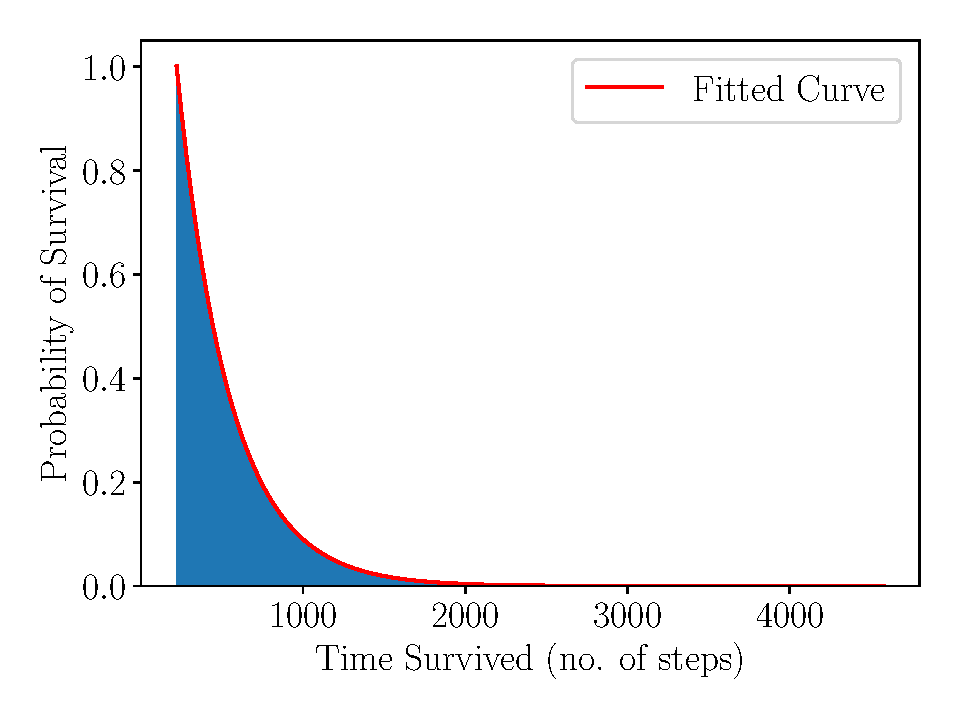
\includegraphics[width=0.5\textwidth]{images/cum_exp_plot.pdf}
  \label{fig:cumhist}}
  \centering
  \subfloat[Histogram of probability of surviving to at least a particular step
  in a logarithmic scale]
  {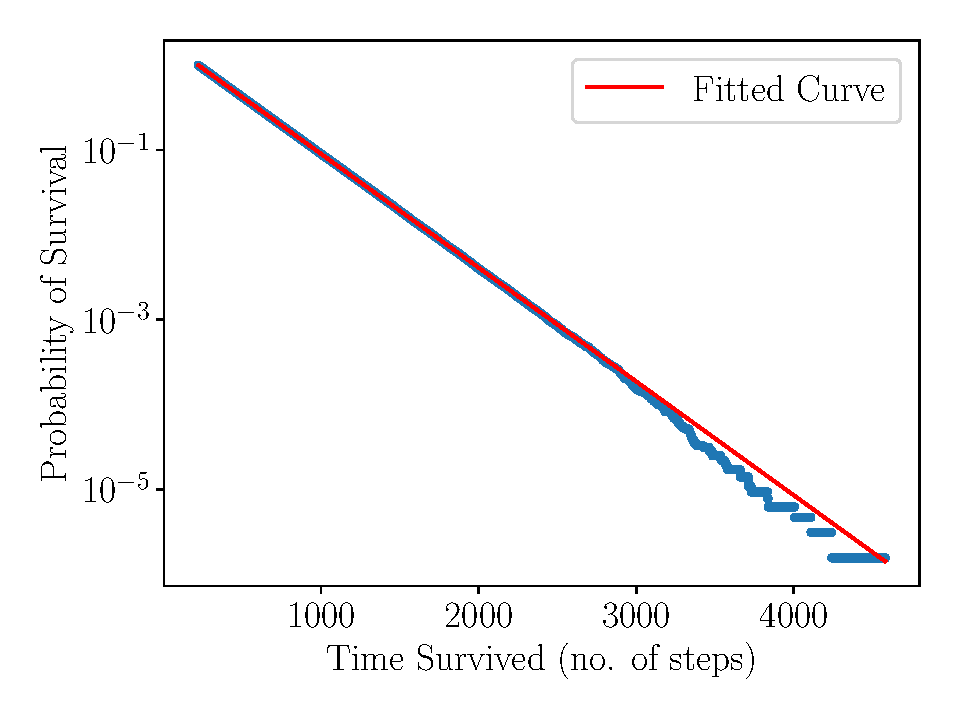
\includegraphics[width=0.5\textwidth]{images/cum_line_plot.pdf}
  \label{fig:cumloghist}}
  \caption{Histogram showing the Probability of surviving to at least a
    particular step in an infinite square well with $J = 20$. The peak of 1 does
    not start at the origin but at step 100. This is because these steps were
    neglected in the plot as prior to this step the exponential shape is less
    clear, as explained by Figure \ref{fig:hist}. An exponential decay curve
    provides a good fit, with an $R^2$ value of 0.9999998, very close to
    1. Plotting on a logarithmic scale shows the straight line fit, the gradient
    of which is $\lambda$, giving $\lambda J^2 = 1.2334$, with a negligible
    error. The fluctuation in the higher step number regions is due to the large
    variance in the small number of walkers that die at these steps.}
  \label{fig:cumplots}
\end{figure*}

The simulation was first run for an infinite square well with boundary $J=20$
with 1000000 walkers. The number of walkers surviving at each step was recorded
and the histograms in Figure \ref{fig:cumplots} were created. The probability
that a walker will survive at a particular step is simply the 1 minus the
normalised cumulative sum of walkers dying at each step. The curve has been
fitted with an exponential function of the form in Equation
\ref{eq:firsteq}. This results in a very good fit, with an $R^2$ value of
0.9999998, indicating the data does not vary much from the curve of best
fit. This is likely due to the very large number of walkers used in this
experiment, as allowed by the performant C++ implementation.

We can see this better in Figure \ref{fig:cumloghist}, which is the same
exponential plot fitted on a logarithmic scale. The closeness of the data to the
line of best fit is evident here. The error in the fitted parameters is
negligible, as shown by the $R^2$ value. The gradient of the fitted line is
taken to be $\lambda$ and thus allows us to calculate $\lambda J^2 = 1.2334$,
compared to the theoretical value of $\frac{\pi^2}{8} = 1.2337$, quoting both
values to the precision at which they vary. Since the numerical error in the
fits is negligible, it cannot be propagated into an error in the final
answer. Thus, we get the error in the final answer from repeated runs of the
simulation and taking the standard deviation of the many values.

As we can observe in Figure \ref{fig:cumhist}, the peak of the curve does not
lie at the origin as we might expect from the fact that all walkers should
survive at least the first step. The reason for this is twofold:
\begin{itemize}
\item For a well with boundary $J$, it is not possible for the walker to die in
  a number of steps less than $J$
\item It is highly unlikely that the walker will die at a number of steps
  greater than but still close to $J$ since it would require walking in the same
  direction a dispropotionate number of times.
\end{itemize}

\begin{figure}%[!ht]
  \begin{center}
    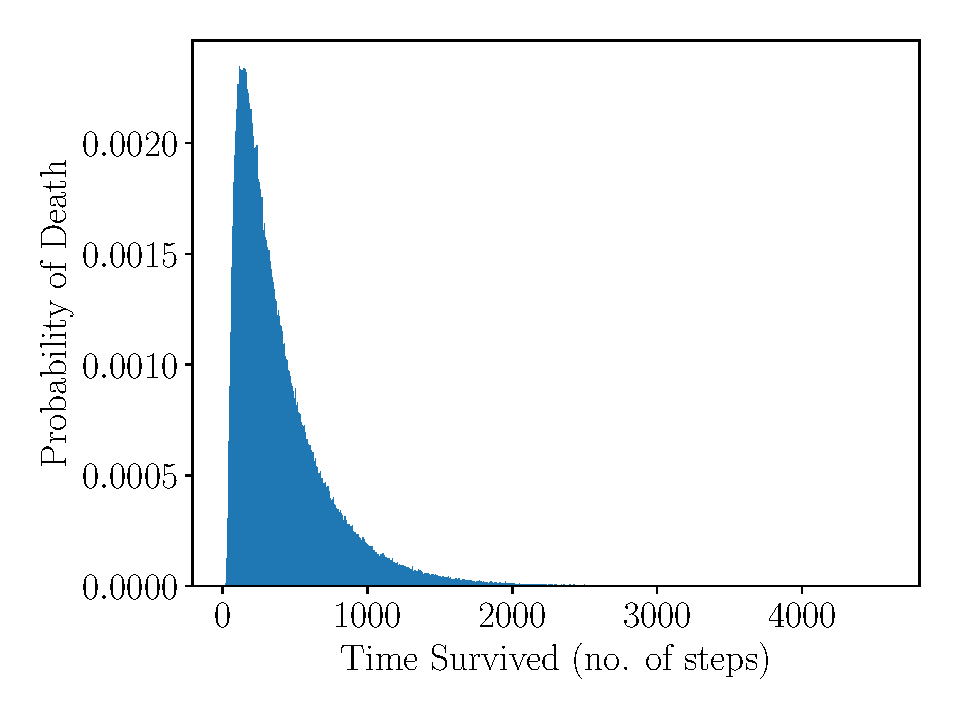
\includegraphics[width=0.45\textwidth]{images/exp_plot.pdf}
    \caption{The probability of dying on a particular step in an infnite square
      well with $J=20$. As can be seen, the peak is away from the origin. This
      is because, for a well with boundary $J$, the minimum number of steps a
      walker must take is $J$. However, it is still unlikely that the walker
      will die on this minimum number of steps, as then the walker must walk in
      the same direction every time. Thus, the most probable step for the walker
      to die on is greater than $J$. It is for this reason that the exponential
      decay does not begin at the origin in Figure \ref{fig:cumhist}, meaning
      some earlier steps must be neglected in order to achieve a better fit.}
    \label{fig:hist}
  \end{center}
\end{figure}

These effects are evident in Figure \ref{fig:hist}, which presents the
probability that a walker will die at a particular number of steps. We can see
that the peak of the curve is very clearly at a step that is greater than 20,
which was the $J$ value used in this simulation. Thus, for low step numbers, the
shape of the curve is not exponential. For this reason we used a simple
algorithm to identify a suitable number of steps to skip before fitting the
exponential curve. It is for this reason that the histogram in Figure
\ref{fig:cumhist} does not start at the origin.


\begin{figure}%[!ht]
  \begin{center}
    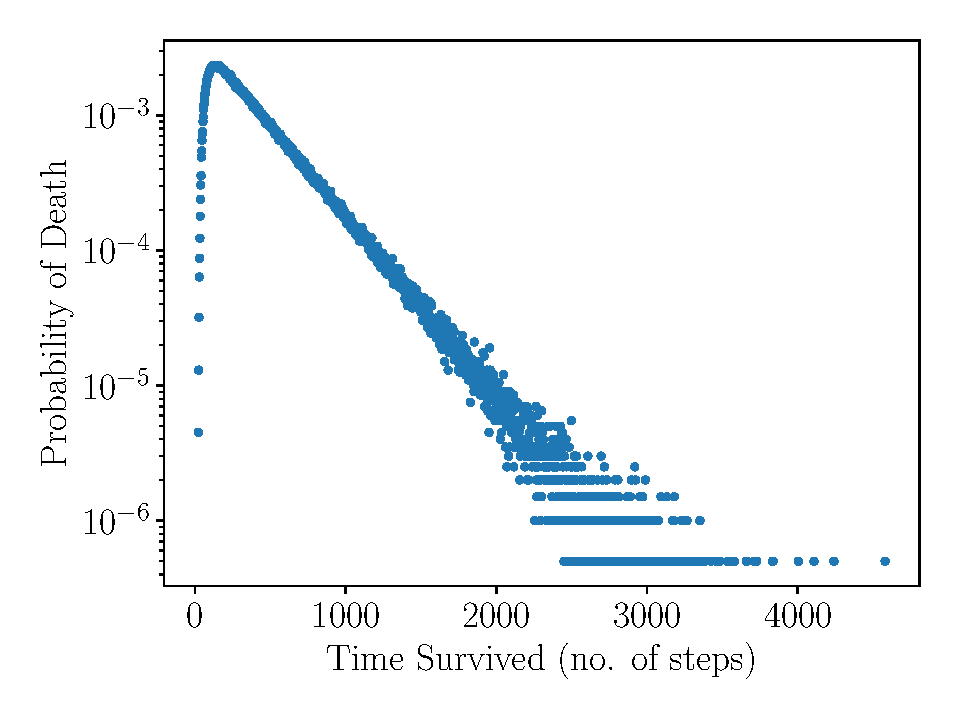
\includegraphics[width=0.45\textwidth]{images/line_plot.pdf}
    \caption{The probability of dying on a particular step in an infnite square
      well with $J=20$, plotted on a logarithmic scale. As explained for Figure
      \ref{fig:hist}, the peak probability is on a step greater than $J$. This
      is clear in this plot. It is also evident that there is significantly more
      spread in the points at higher steps. This is due to there being
      significantly fewer walkers dying on these steps, so the relative
      differences are higher. This explains the fluctuations seen at higher
      steps in Figure \ref{fig:cumloghist}.}
    \label{fig:loghist}
  \end{center}
\end{figure}

We observe some fluctuation in the data in the higher steps in Figure
\ref{fig:cumloghist}. This is because there are so few walkers surviving to this
many steps that there is more significant variance in their relative numbers. We
can observe this in Figure \ref{fig:loghist}. At higher step numbers, the spread
is clearly larger due to the greater relative variance in the small number of
walkers surviving to this many steps. When this data is cumulatively summed to
calculate the probability of survival shown in Figure \ref{fig:cumloghist}, the
spread is present as the fluctuations.

\begin{figure*}%[ht!]
  \centering
  \subfloat[Probability of dying on a particlar step with a step cutoff]
  {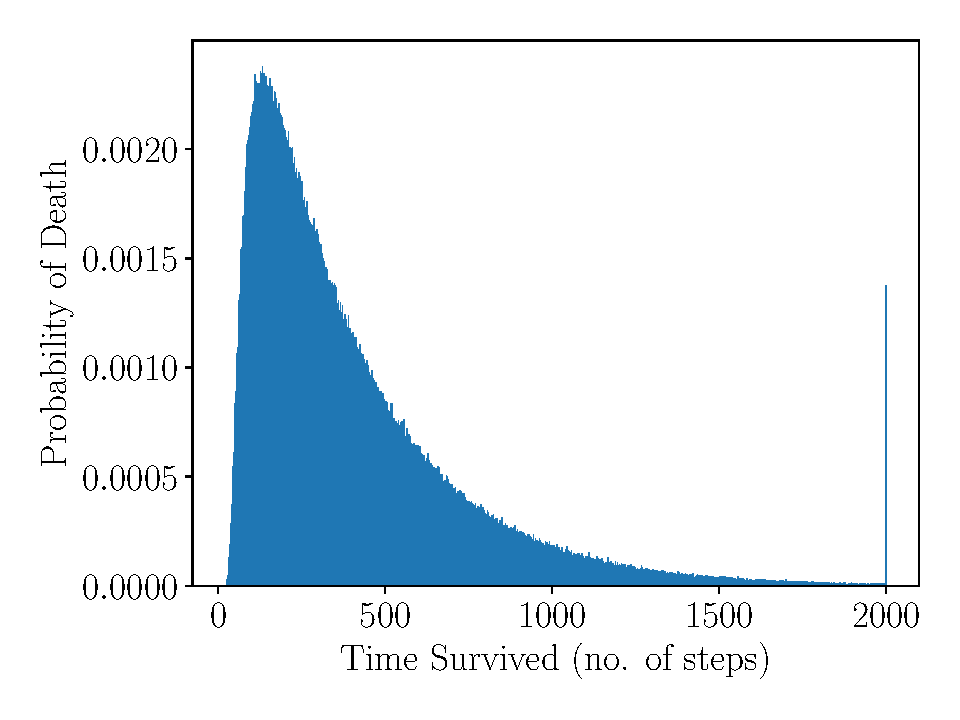
\includegraphics[width=0.5\textwidth]{images/exp_plot_cutoff.pdf}
  \label{fig:expcutoff}}
  \centering
  \subfloat[Probability of surviving to at least a particular step in a
  logarithmic scale with a step cutoff]
  {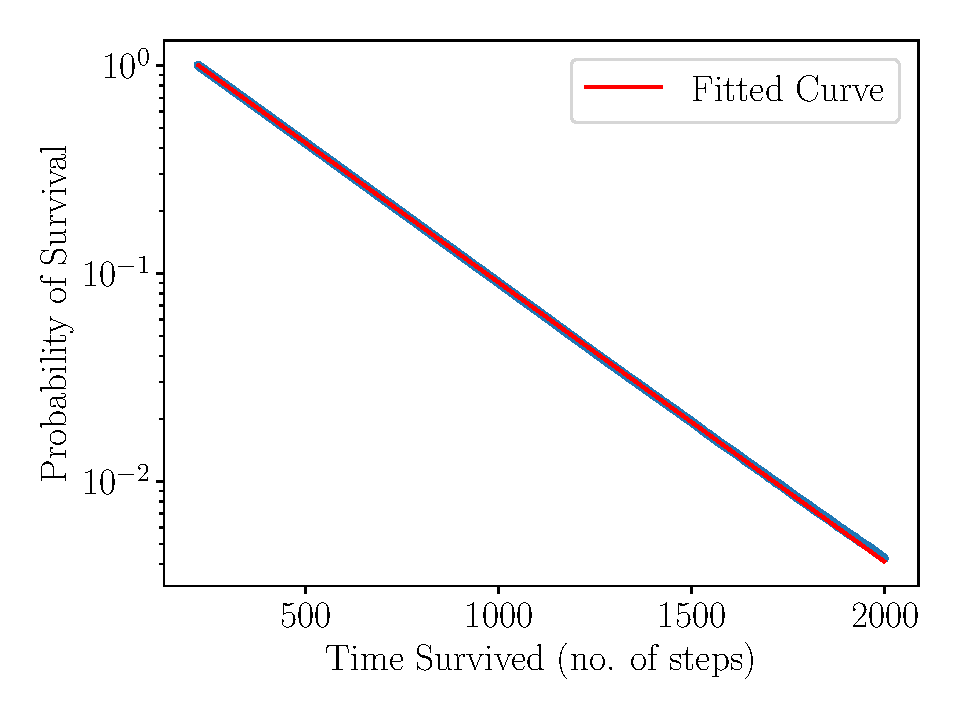
\includegraphics[width=0.5\textwidth]{images/cum_line_plot_cutoff.pdf}
  \label{fig:cum_line_cutoff_plot}}
  \caption{Histograms showing the results of the simulation when a maximm number
  of steps is introduced. If a walker reaches this number of steps, they
  automatically die, regardless of position. This results in a
  disproportionately high number of walkers dying at this maximum number, 2000
  in this case, as shown by Figure \ref{fig:expcutoff}. However, this results in
  no fluctuation at higher number of steps, as shown in Figure
  \ref{fig:cum_line_cutoff_plot}, though some systematic error is introduced
  through this method.}
  \label{fig:cutoffplots}
\end{figure*}

It is possible to remove this variance by introducing a cutoff number of steps,
i.e. a maximum number of steps at which the walker will automatically die,
regardless of whether they reached a boundary or not. Thus, there will not be
such high variance in the number of walkers surviving to high number of
steps. This is presented in Figure \ref{fig:cum_line_cutoff_plot}. While this
fit is observed to be better, with a higher $R^2$ value, some systematic error
has been introduced since there will now be a disproportionately high number of
walkers dying at the cutoff step as can be seen in Figure
\ref{fig:expcutoff}. Thus, the final $\lambda J^2$ value will be less
accurate. On a faster computer, with more efficient code, it is possible to
forgo the step cutoff and allow the simulation to run until all the walkers
die. This may take much longer but will ensure there will not be such a
systematic error introduced. This is the method used in this investigation.


It is also necessary to investigate how varying the boundary $J$ affects the
accuracy of the final answer. Figure \ref{fig:multi_line_plot} presents the
cumulative summed histograms with their fitted lines for many different boundary
$J$ values. No step cutoff was introduced. The calculated $\lambda J^2$ value is
shown in the legend. As shown, the gradient changes, but this is to be expected
since the expected highest number of steps would increase as the boundary is
larger, since there is more space for the walker to move before reaching a
boundary. As shown in the legend, the calculated $\lambda J^2$ values get closer
and closer and closer to the theoretical value as $J$ increases. This is due to
the fact that as $J$ increases, there are more walkers surviving to larger
number of steps. Thus, we can say that using a larger value of $J$ will result
in a more accurate answer but will also be more computationally intensive and
take longer. Thus, we make a tradeoff between speed and accuracy and choose
$J=20$ for the final investigation.

Running the simulation 10 times and taking the average $\lambda J^2$ with error
being standard deviation, we find:
\begin{equation}
  \lambda J^2 = 1.2339 \pm 0.0008
  \nonumber
\end{equation}
We quote the precision to the decimal place at which there is variation from the
theoretical result of $1.2337$. We notice that the error in the calculated
answer is small (since there is not much variation between repeated simulations)
and the theoretical result is within the range of the calculated answer.


\todo{circular well}

\begin{figure}%[!ht]
  \begin{center}
    \includegraphics[width=0.45\textwidth]{images/multiplot1.pdf}
    \caption{Histogram plotted on a logarithmic scale showing the Probability of
      surviving to at least a particualr step in different infinite square wells
      with different boundaries $J$. The simulations were run with $10000$
      walkers The $\lambda J^2$ values for each are shown. The values get closer
      to the theoretical value of $\frac{\pi^2}{8} = 1.2337$ as we increase the
      size of the well. This is likely due to more walkers surviving to a higher
      number of steps, as the well size is increased.}
    \label{fig:multi_line_plot}
  \end{center}
\end{figure}


\section{Conclusions}

In this investigation we demonstrated a method of calculating ground state
energies of a quantum system using Random walk computational simulations. The
investigation focussed on an Infinite Square Well, but is easily extended to a
Symmetric potential. The simualation was written in C++ to maximise performance
and is available at \todo{cite}.

The investigation explored the effects of varying the size of the well in
determining the ground state energy of a quantum system, and showed that this
method is more effective for larger wells, i.e. wells with larger
boundaries. This is because for wells with larger boundaries, the walker can
take a larger number of steps on average before dying, and thus can populate
larger step bins. Thus, this method produces data that is close to the
theoretical result for larger infinite square wells.

The general theoretical result for the ground state energy of an infinite square
well is $\frac{\pi^2}{8}\frac{\hbar^2}{mJ^2}$ where $J$ is the boundary of the
well, and this method allows for the calculation of $\lambda R^2
\frac{\hbar^2}{mJ^2}$, where $R$ also corresponds to the boundary of the
well. Thus, we expect our calculated result to be $\lambda R^2 = \lambda J^2 =
\frac{\pi^2}{8}$.

This method provided $\lambda J^2 = 1.2339 \pm 0.0008$, which lies within the
range of the theoretical result.

This method can be easily extended to multiple dimensions with only a linear
increase in time complexity for each added dimension. Thus, while this method
may not be very efficient for low number of dimensions, it quickly becomes
effective at a higher number of dimensions.


\appendices
\section{Random walk Schr\"{o}dinger Equation Derivation}
\label{appendix:derivation}
Consider a one-dimensional lattice upon which a walker is undergoing a random
walker. Let us denote the probability that the walker is at position $j$ after
$n$ steps as $p(j,n)$ and the probabilty that the walker will die at position
$j$ as $a(j)$. We will denote the position-step number coordinates as $[j,
n]$. Thus, for a walker to have coordinates $[j, n+1]$, in the previous step,
they must have had coordinates $[j \pm 1, n]$. So we can say:

\begin{equation}
  \label{eq:probability}
  p(j, n+1) =  \frac{1}{2}(1-a(j))(p(j-1,n) + p(j+1,n))
\end{equation}

If $a(j)$ is small and $n$ is large, then we can say $p(j, n)$ is a continuous
function and we can use Taylor expansion to expand each of $p(j+1, n)$,
$p(j-1,n)$, and $p(j, n+1)$:

\begin{equation}
  p(j+1, n) = p(j,n) + \frac{\partial p}{\partial j} + \frac{1}{2}
  \frac{\partial^2 p}{\partial j^2} + ...
  \nonumber
\end{equation}
\begin{equation}
  p(j-1, n) = p(j,n) - \frac{\partial p}{\partial j} + \frac{1}{2}
  \frac{\partial^2 p}{+\partial j^2} + ...
  \nonumber
\end{equation}
\begin{equation}
  p(j, n+1) = p(j, n) + \frac{\partial p}{\partial n} + ...
  \nonumber
\end{equation}

We can now substitute these expansions into Equation \ref{eq:probability}, we
find:

\begin{equation}
  p(j, n) + \frac{\partial p}{\partial n} = (1-a(j))\Big(p +
  \frac{1}{2}\frac{\partial^2 p}{\partial j^2}\Big)
  \nonumber
\end{equation}

But the probability of death $a(j)$ and the second derivative are so small, that
their product is neglected. We also let $p(j,n) = q(j) \exp(-\lambda n)$ so that:

\begin{equation}
  -\frac{1}{2} \frac{d^2q(j)}{dj^2} + a(j)q(j) = \lambda q(j)
  \nonumber
\end{equation}

\printbibliography

\end{document}


